\pgfplotstablegetelem{\thepart}{[index]\columnIndex}\of{\cronograma}
\part{\pgfplotsretval}
\label{part:\thepart}
\frame{\partpage}


\begin{frame}[t]{Padrões de desenvolvimento de software}
	
	\fontsize{12pt}{15.2}\selectfont{
		...continuando Padrões de desenvolvimento de software.\\ 
	}\par
	\vspace{1em}
	
	
	\fontsize{12pt}{15}\selectfont{
		\begin{itemize}%[<+->]  
			
			\item {\color{red}Padrões de Criação.}
			
			\begin{itemize}%[<+->]
				\item {\color{blue}Singleton \CheckmarkBold}
				\item {\color{blue}Abstract Factory \CheckmarkBold}
				\item Factory Method \XSolidBrush
				\item Builder \XSolidBrush
				\item Prototype \XSolidBrush
			\end{itemize}
			
		\end{itemize}
	}\par
	\vspace{1em}
	
	
\end{frame}




\begin{frame}[t]{Padrões de criação}
	\fontsize{12pt}{15.2}\selectfont{
		{\color{blue}Factory Method \CheckmarkBold}
	}\par
	\vspace{1em}

	\fontsize{12pt}{15}\selectfont{
		\begin{itemize}%[<+->]  

			\item Padrão que define um método para criar um objeto em uma classe-mãe, mas permite que subclasses modifiquem o tipo de objeto que será criado.
			
			\item Ele é ideal quando você tem uma superclasse que faz algo, mas quer que subclasses específicas decidam como criar esses objetos.

		\end{itemize}
	}\par
	\vspace{1em}
\end{frame}








\begin{frame}[t]{Padrões de criação}
	\fontsize{12pt}{15.2}\selectfont{
		Exemplo
	}\par
	\vspace{1em}
	
	\fontsize{12pt}{15}\selectfont{
		\begin{itemize}%[<+->]  
			
			\item Imagine que você tenha uma classe Documento que é responsável por abrir arquivos. 
			
			\item Dependendo do tipo de documento (PDF, Word), você quer abrir o documento de maneiras diferentes. 
			
			\item O \textbf{Factory Method} permite que cada tipo de documento implemente seu próprio método de abertura.
			
		\end{itemize}
	}\par
	\vspace{1em}
\end{frame}




\begin{frame}[t]{Padrão de projeto Factory Method}

	\lstinputlisting[style=CBruno,caption=Código da Classe Documento - codigo\_016\_documento\_abstrata.py Abstrata]{outros/codigos/python/exemplos-de-aulas/src/codigo_016_documento_abstrata.py}

\lstinputlisting[style=CBruno,caption=Código da Classe Documento Pdf - codigo\_016\_documento\_pdf\_concreta.py Concreta]{outros/codigos/python/exemplos-de-aulas/src/codigo_016_documento_pdf_concreta.py}

\lstinputlisting[style=CBruno,caption=Código da Classe Documento Ms Word - codigo\_016\_documento\_msword\_concreta.py Concreta]{outros/codigos/python/exemplos-de-aulas/src/codigo_016_documento_msword_concreta.py}


\end{frame}


\begin{frame}[t]{Padrão de projeto Factory Method}
	
	\lstinputlisting[style=CBruno,caption=Código da função codigo\_cliente\_factory\_method]{outros/codigos/python/exemplos-de-aulas/src/codigo_016_codigo_cliente_factory_method.py}


*obs: Linhas de 1 a 6 são para ajustar a leitura dos arquivos para o Phyton, que estão no mesmo diretório.

\end{frame}


\begin{frame}[t]{Padrão de projeto Factory Method}
	
	\lstinputlisting[style=CBruno,caption=Testes do Código do cliente para utilizar a Factory Method - test\_codigo\_016\_cliente\_factory\_method.py ]{outros/codigos/python/exemplos-de-aulas/tests/test_codigo_016_cliente_factory_method.py}


\end{frame}




\begin{frame}[t]{Padrão de projeto Factory Method}
	
	\lstinputlisting[style=CBruno,caption=Código da Classe Documento Factory Method Concreta  - codigo\_016\_documento\_factory\_method\_concreta.py]{outros/codigos/python/exemplos-de-aulas/src/codigo_016_documento_factory_method_concreta.py}

*obs: quaias as vantagens e desvantagens desta "segunda" implementação? que utilizou a classe \textbf{DocumentoFactoryMethodConcreta}.

\end{frame}



\begin{frame}[t]{Padrão de projeto Factory Method}
	
	\lstinputlisting[style=CBruno,caption=Código do cliente para utilizar a Factory Method - codigo\_016\_codigo\_cliente\_factory\_method2.py ]{outros/codigos/python/exemplos-de-aulas/src/codigo_016_codigo_cliente_factory_method2.py}
	
\end{frame}


\begin{frame}[t]{Padrão de projeto Factory Method}
	
	\lstinputlisting[style=CBruno,caption=Testes do Código do cliente para utilizar a Factory Method ]{outros/codigos/python/exemplos-de-aulas/tests/test_codigo_016_cliente_factory_method2.py}
	
\end{frame}





\begin{frame}[t]{Padrões de criação}
	\fontsize{12pt}{15.2}\selectfont{
		Diferenças Fundamentais entre Abstract Factory e Factory Method?
	}\par
	\vspace{0.5em}
	
	\fontsize{12pt}{13}\selectfont{
		\begin{itemize}%[<+->]
			
			\item \textbf{Escopo de Aplicação}
			\begin{itemize}%[<+->]
				\item Abstract Factory: Focado na criação de famílias de objetos relacionados.
				\item Factory Method: Focado na criação de um único objeto, delegando a subclasses a decisão de qual tipo de objeto criar.
			\end{itemize}
				
			\item \textbf{Complexidade}
			\begin{itemize}%[<+->]
				\item Abstract Factory: Envolve várias classes e métodos para criar diferentes objetos relacionados.
				\item Factory Method: Mais simples, envolvendo um único método de criação.
			\end{itemize}
			
			\item \textbf{Flexibilidade}
			\begin{itemize}%[<+->]
				\item Abstract Factory: Útil para criar produtos consistentes entre si.
				\item Factory Method: Útil quando a criação de objetos pode variar em subclasses.
			\end{itemize}

		\end{itemize}
	}\par
	\vspace{1em}
\end{frame}



\begin{frame}[t]{Abstract Factory}
	\vspace{1em}
	\centering
	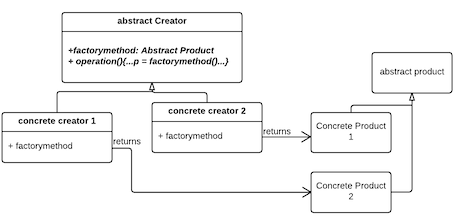
\includegraphics[scale=1.25]{imagens/fig-factory-method-diagram.png}
	
\end{frame}


